\section{Suddivisione del lavoro}
Vengono qui di seguito descritti i ruoli ricoperti dai vari membri del gruppo durante lo svolgimento del progetto.
\subsection{Investimento non rendicontato}
\subsubsection{\AR}
Nel periodo di \AR{} ciascun componente dovrà ricoprire i seguenti ruoli e per la quantità di ore specificate:


I valori sono riassunti nel seguente grafico, che rappresenta in maniera visiva per quante ore un membro ricoprirà un determinato ruolo.
\begin{figure}[H]
	\centering
	\includegraphics[width=14cm]{img_suddlavoro/AA.png}
	\caption{Ore per componente, periodo di \AR{}}
\end{figure}

\subsection{Investimento Rendicontato}
\subsubsection{\AD}
Nel periodo di \AD{} ciascun componente dovrà ricoprire i seguenti ruoli e per la quantità di ore specificate:


I valori sono riassunti nel seguente grafico, che rappresenta in maniera visiva per quante ore un membro ricoprirà un determinato ruolo.
\begin{figure}[H]
	\centering
	\includegraphics[width=14cm]{img_suddlavoro/AD.png}
	\caption{Ore per componente, periodo di \AD{}}
\end{figure}

\subsubsection{\PA}
Nella periodo di \PA{} ciascun componente dovrà ricoprire i seguenti ruoli e per la quantità di ore specificate:


I valori sono riassunti nel seguente grafico, che rappresenta in maniera visiva per quante ore un membro ricoprirà un determinato ruolo.
\begin{figure}[H]
	\centering
	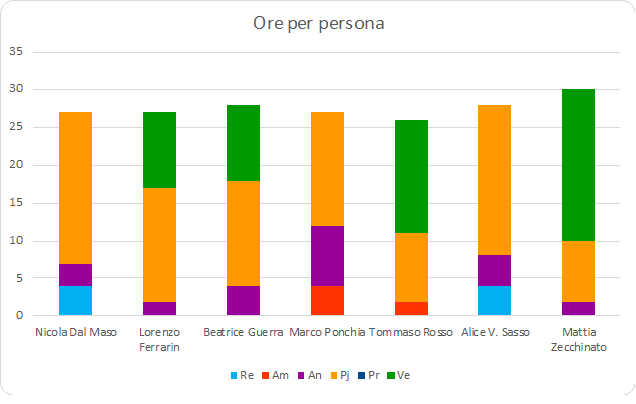
\includegraphics[width=14cm]{img_suddlavoro/PA.png}
	\caption{Ore per componente, periodo di \PA{}}
\end{figure}

\subsubsection{\PD}
Nel periodo di \PD{} ciascun componente dovrà ricoprire i seguenti ruoli e per la quantità di ore specificate:

I valori sono riassunti nel seguente grafico, che rappresenta in maniera visiva per quante ore un membro ricoprirà un determinato ruolo.
\begin{figure}[H]
	\centering
	\includegraphics[width=14cm]{img_suddlavoro/PD.png}
	\caption{Ore per componente, periodo di \PD{}}
\end{figure}

\subsubsection{\Cod}
Nel periodo di \Cod{} ciascun componente dovrà ricoprire i seguenti ruoli e per la quantità di ore specificate:

I valori sono riassunti nel seguente grafico, che rappresenta in maniera visiva per quante ore un membro ricoprirà un determinato ruolo.
\begin{figure}[H]
	\centering
	\includegraphics[width=14cm]{img_suddlavoro/C.png}
	\caption{Ore per componente, periodo di \Cod{}}
\end{figure}

\subsubsection{\VV}
Nel periodo di \VV{} ciascun componente dovrà ricoprire i seguenti ruoli e per la quantità di ore specificate:
}
I valori sono riassunti nel seguente grafico, che rappresenta in maniera visiva per quante ore un membro ricoprirà un determinato ruolo.
\begin{figure}[H]
	\centering
	\includegraphics[width=14cm]{img_suddlavoro/VV.png}
	\caption{Ore per componente, periodo di \VV{}}
\end{figure}

\subsection{Totale}
\subsubsection{Ore totali con investimento}
Le ore totali, comprese quelle investite in analisi, divise per componente durante il progetto saranno le seguenti:


%I valori sono riassunti nel seguente grafico, che rappresenta in maniera visiva per quante ore un membro ricoprirà un determinato ruolo.
%\begin{figure}[H]
%	\centering
%	\includegraphics[width=14cm]{img_suddlavoro/TOT.png}
%	\caption{Ore totali per componente}
%\end{figure}

\subsubsection{Ore totali senza investimento}
Le ore totali rendicontate, cioè quelle senza investimento iniziale, divise per componente durante il progetto saranno le seguenti:


I valori sono riassunti nel seguente grafico, che rappresenta in maniera visiva per quante ore un membro ricoprirà un determinato ruolo.
\begin{figure}[H]
	\centering
	\includegraphics[width=14cm]{img_suddlavoro/TOT.png}
	\caption{Ore totali per componente}
\end{figure}





